\documentclass[10pt]{beamer}
\usetheme{AGH}

\usepackage{lmodern}
\usepackage[utf8]{inputenc}
\usepackage{listings} 
\usepackage{siunitx}
\usepackage{filecontents,hyperref}
\usepackage{graphicx}
\usepackage{subcaption}
\usepackage{svg}

\usepackage{appendixnumberbeamer}
\usepackage{booktabs}
\usepackage{xspace}
\newcommand{\themename}{\textbf{\textsc{metropolis}}\xspace}


\title{Drzewa wszystkich najkrótszych ścieżek - algorytm Dijkstry}
\subtitle{\normalsize{Aplikacja PGAS}}
\date{}
\author{\normalsize{Arkadiusz Kasprzak, Aleksandra Poręba}}



\definecolor{lgray}{gray}{0.96}
\definecolor{lbcolor}{rgb}{0.9,0.9,0.9}
\lstset{
    framesep=2pt,
    basicstyle=\ttfamily,
    breaklines=true,
    breakatwhitespace=true,
    aboveskip={0.75\baselineskip},
    columns=fixed,
    showstringspaces=false,
    breaklines=true,
    prebreak = \raisebox{0ex}[0ex][0ex]{\ensuremath{\hookleftarrow}},
    frame=single,
    rulecolor=\color{lgray},
    showtabs=false,
    showspaces=false,
    showstringspaces=false,
    backgroundcolor=\color{lgray},
    identifierstyle=\ttfamily,
    keywordstyle=\color[rgb]{0,0,1},
    commentstyle=\color[rgb]{0.0,0.26,0.15},
    stringstyle=\color[rgb]{0.627,0.126,0.941}
}


\begin{document}

\titleframe[pl]

\begin{frame}
\frametitle{Agenda}
\tableofcontents
\end{frame}

\section{Algorytm Dijkstry - wprowadzenie}

\begin{frame}
\frametitle{Algorytm Dijkstry - wprowadzenie}
\begin{itemize}
\item Cel: znalezienie najkrótszych ścieżek z wybranego wierzchołka grafu do wszystkich pozostałych wierzchołków.
\item Operujemy na grafie skierowanym lub nieskierowanym o nieujemnych wagach krawędzi.
\item Algorytm zachłanny - w każdym kroku algorytmu wybierany jest wierzchołek o najmniejszej wartości kosztu.
\item Możliwość znalezienia zarówno najkrótszych ścieżek, jak i ich kosztów.
\end{itemize}
\end{frame}

\section{Budowa i działanie projektu}

\begin{frame}
\frametitle{Działanie projektu - wprowadzenie}
Program podzielony został na części:
\begin{itemize}
\item wczytanie danych wejściowych,
\item zapis kolumn do sąsiedztwa odpowiednich procesów,
\item obliczanie odległości i ścierzek - algorytm Dijkstry,
\item zapisy wyników do pliku oraz zakończenie.
\end{itemize}

Szczegółowy opis wraz ze schematami blokowymi zawarty został w dokumentacji projektu.
\end{frame}

\begin{frame}
\frametitle{Działanie projektu - dane wejściowe}
\begin{itemize}
\item Dane podawane w postaci tzw. macierzy sąsiedztwa.
\item Są one wczytywane z pliku przez proces o numerze 0.
\end{itemize}
\begin{figure}
\centering
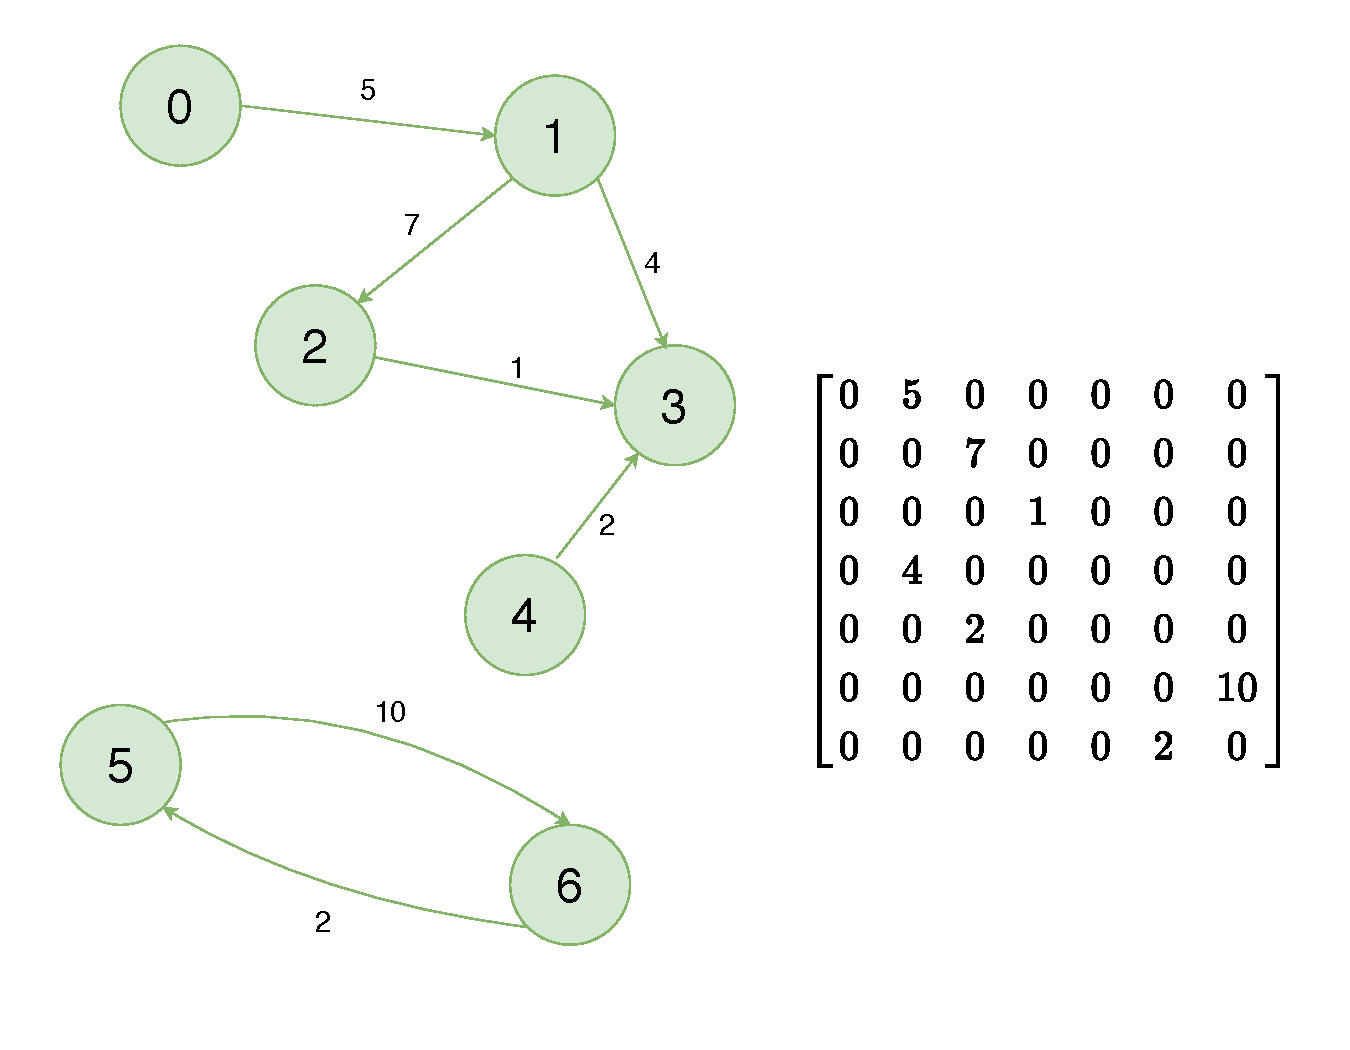
\includegraphics[width=0.7\textwidth]{static/Example.pdf}
\end{figure}

\end{frame}

\begin{frame}
\frametitle{Działanie projektu - podział danych wejściowych}
\begin{itemize}
\item Dane dzielone są kolumnami równomiernie pomiędzy wszystkie procesy. 
\item Jeśli podział równomierny jest niemożliwy, pozostałe $k$ kolumn dzielone jest między pierwsze $k$ procesów.
\item Procesy otrzymują kolumny o indeksach  \\ 
\begin{center} 
\textit{ indeks\_kolumny mod liczba\_procesów == numer\_procesu}
\end{center}

\end{itemize}
\begin{figure}
\centering
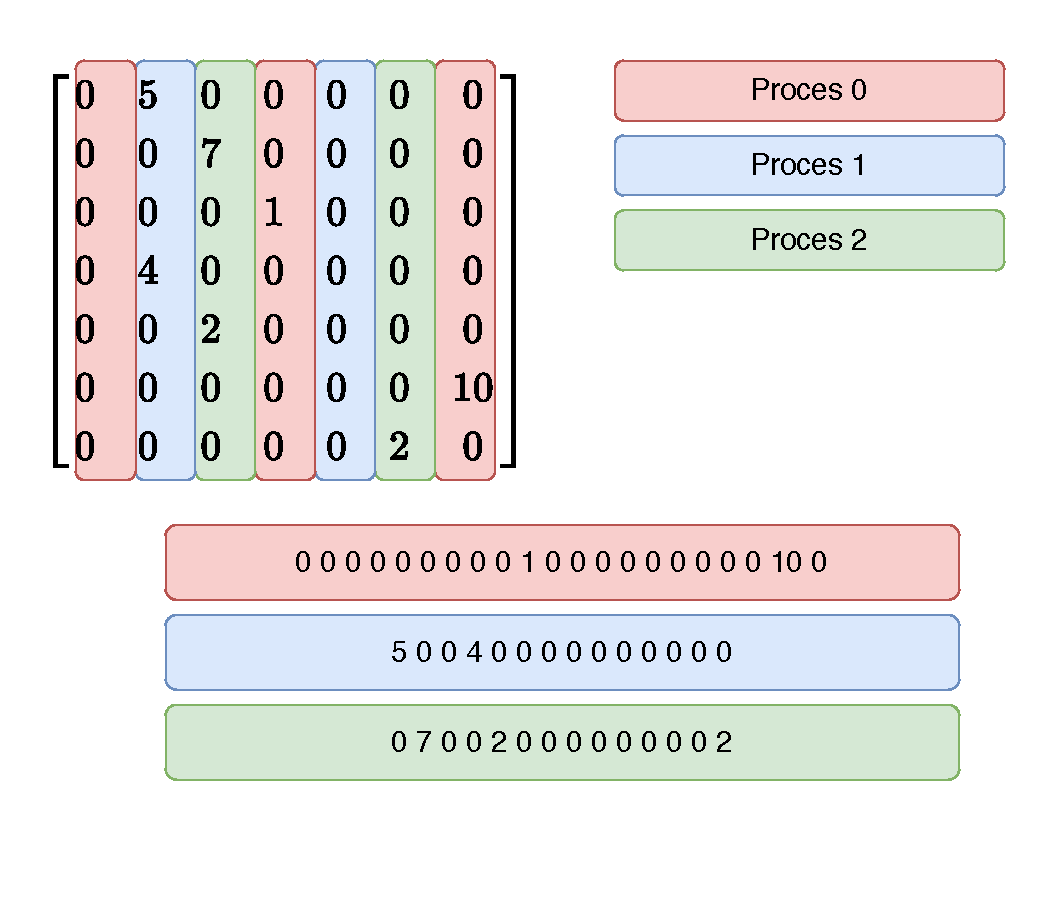
\includegraphics[width=0.4\textwidth]{static/MatrixChunks.pdf}
\end{figure}
\end{frame}

\begin{frame}
\frametitle{Działanie projektu - przebieg algorytmu}
\begin{itemize}
\item Operujemy na trzech tablicach: tablicy kosztów, tablicy poprzedników, oraz tablicy informującej, czy wierzchołek został już przetworzony.
\item Są one współdzielone pomiędzy procesami, ale każdy z nich będzie wypełniał pozycje tylko dla wierzchołków w jego sąsiedztwie.
\item Tablica kosztów inicjalizowana nieskończonościami, tablica poprzedników - wartościami -1, a tablica przetworzonych zerami.
\item Koszt dla wierzchołka źródłowego ustawiany na 0.
\end{itemize}
\begin{figure}
\centering
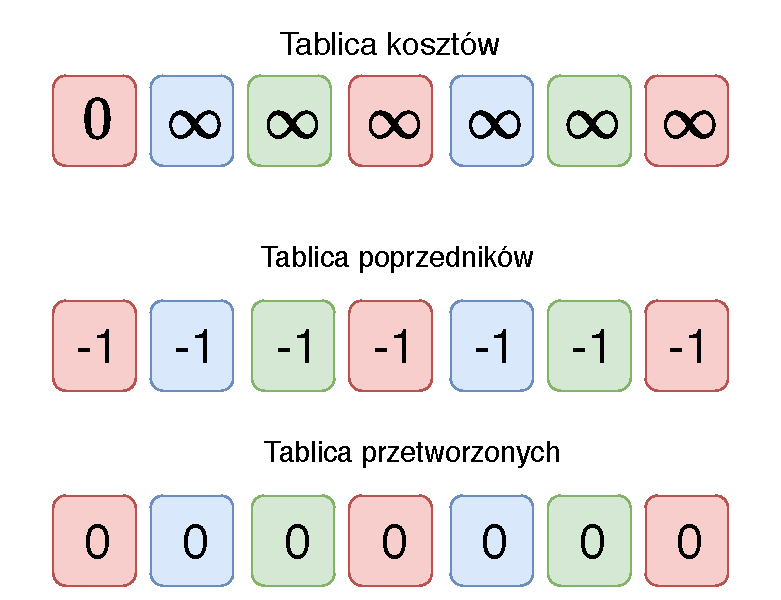
\includegraphics[width=0.35\textwidth]{static/Arrays.pdf}
\caption{Przykładowy początkowy stan tablic}
\end{figure}
\end{frame}

\begin{frame}
\frametitle{Działanie projektu - przebieg algorytmu}
W dalszej części programu powtarzamy poniższe czynności aż wszystkie wierzchołki zostaną przetworzone:
\begin{itemize}
\item każdy proces spośród przydzielonych mu nieprzetworzonych jeszcze wierzchołków wybiera ten o najmniejszej wartości kosztu
\item spośród wszystkich odległości wybierana jest ta najmniejsza (operacja \lstinline{upc_all_reduce}). Odnajdowany zostaje indeks wierzchołka i zostaje on zaznaczony jako przetworzony
\item na podstawie wylosowanego wierzchołka przeprowadzana jest aktualizacja w tabelach kosztów i poprzedników
\end{itemize}
Po zakończeniu działania algorytmu wyniki algorytmu zapisywane są przez proces 0 do pliku.
\end{frame}

\begin{frame}
\frametitle{Działanie projektu - przebieg pojedynczej pętli}
\begin{tabular}{cl}  
         \begin{tabular}{c}
           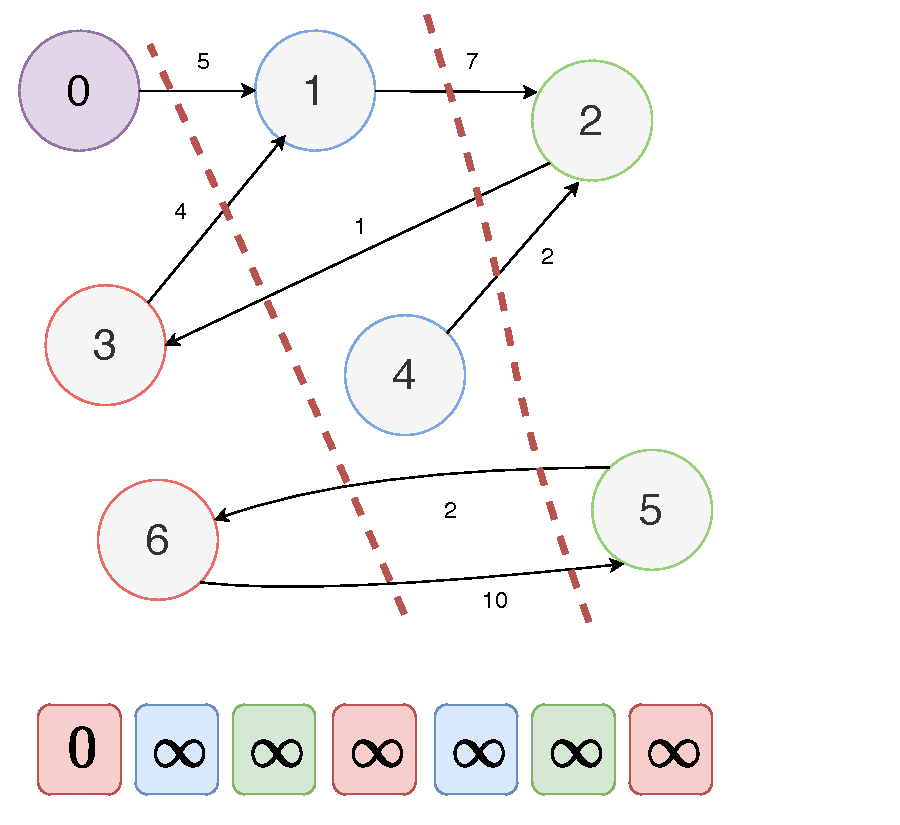
\includegraphics[width=0.5\textwidth]{static/Algo0.pdf}
           \end{tabular}
           & \begin{tabular}{l}
             \parbox{0.4\textwidth}{
		Sytuacja początkowa. Na fioletowo został zaznaczony wierzchołek źródłowy. Czerwoną linią pokazany został podział grafu między procesy. Na dole znajduje się tablica kosztów.

    }
         \end{tabular}  \\
\end{tabular}
\end{frame}

\begin{frame}
\frametitle{Działanie projektu - przebieg pojedynczej pętli}
\begin{tabular}{cl}  
         \begin{tabular}{c}
           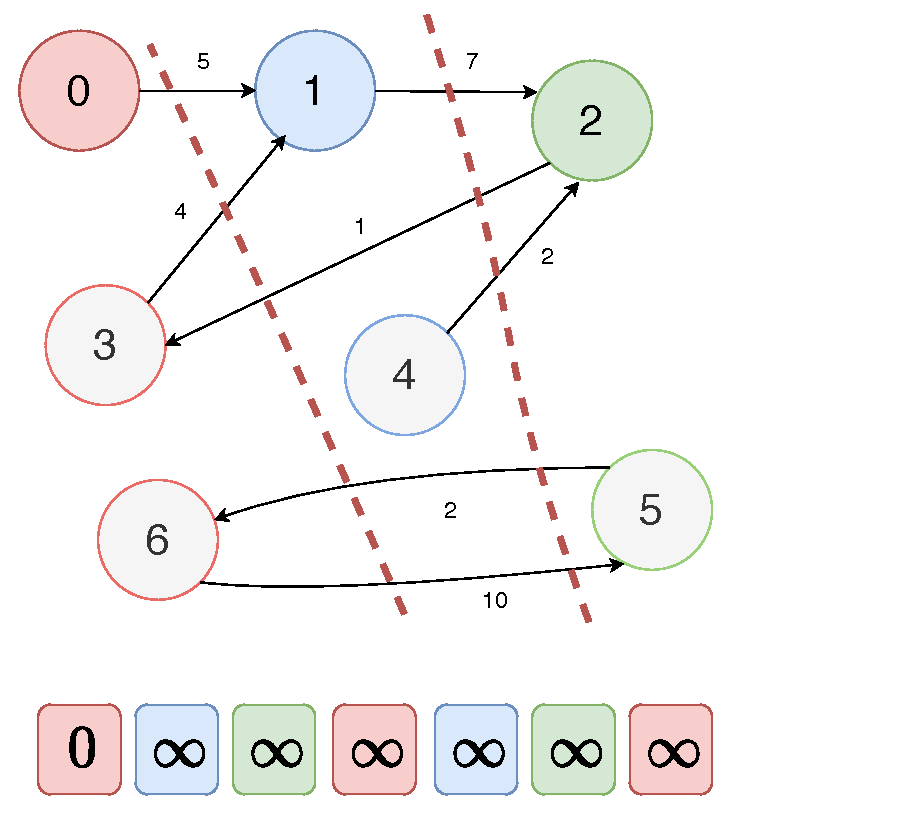
\includegraphics[width=0.5\textwidth]{static/Algo1.pdf}
           \end{tabular}
           & \begin{tabular}{l}
             \parbox{0.4\textwidth}{
		Wybór nieprzetworzonych wierzchołków o najniższym koszcie dotarcia (w tablicy) w każdym z procesów.
    }
         \end{tabular}  \\
\end{tabular}

\end{frame}

\begin{frame}
\frametitle{Działanie projektu - przebieg pojedynczej pętli}
\begin{tabular}{cl}  
         \begin{tabular}{c}
           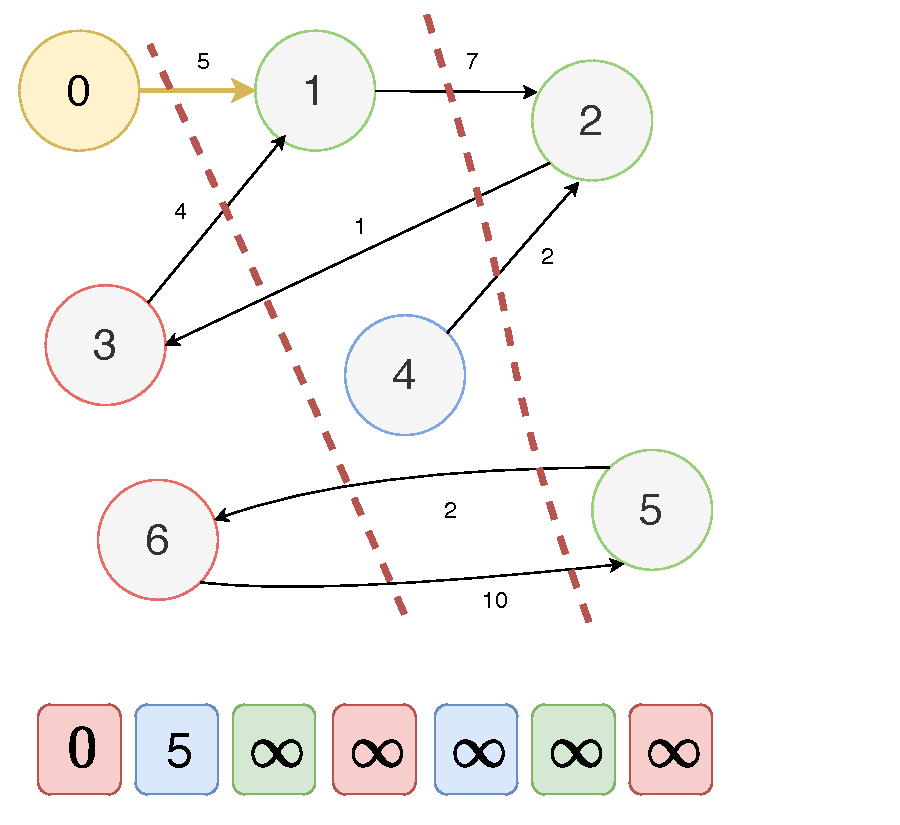
\includegraphics[width=0.5\textwidth]{static/Algo2.pdf}
           \end{tabular}
           & \begin{tabular}{l}
             \parbox{0.4\textwidth}{
		Wybór wierzchołka o globalnie najniższym koszcie (\lstinline{upc_all_reduce}) i zaznaczenie go jako przetworzony. Aktualizacja kosztów i poprzedników.
    }
         \end{tabular}  \\
\end{tabular}
\end{frame}

\begin{frame}[fragile]
\frametitle{Interfejs}
\begin{itemize}
\item Podział grafu pomiędzy poszczególne procesy jest przedstawiany użytkownikowi.
\end{itemize}
\begin{lstlisting}[basicstyle=\tiny]
Proces 0 posiada 4 kolumn o indeksach:  0,  3,  6,  9,
Proces 1 posiada 3 kolumn o indeksach:  1,  4,  7,
Proces 2 posiada 3 kolumn o indeksach:  2,  5,  8,
\end{lstlisting}

\end{frame}

\section{Kompilacja i uruchomienie}

\begin{frame}
\frametitle{Kompilacja i uruchomienie}
\begin{itemize}
\item Przejście do katalogu \lstinline{build_uni}
\item Przygotowanie środowiska pracowni za pomocą skryptu \lstinline{setup.sh}
\item Wykonanie polecenia \lstinline{make}
\item Wykonanie polecenia \lstinline{make run} z opcjonalnymi argumentami określającymi: plik z węzłami, ilość procesów, numer wierzchołka źródłowego oraz ścieżkę do pliku z danymi
\item Wynik dostępny w pliku \lstinline{resultsUPC.txt}
\item Proces szczegółowo opisany w dokumentacji
\end{itemize}

\end{frame}

\end{document}